\section{Setup: a controlled $2 \times 2$}
\label{sec:setup}

\textbf{Task, simulator, reward.} The therapist is \texttt{Llama-3.2-1B} (bf16, LoRA $r{=}16$,
$\alpha{=}16$, lr $1\mathrm{e}{-}5$, seed 42). The patient is \texttt{gpt-4o-mini} conditioned on
one of \textbf{96} persona system prompts, enumerated exhaustively as $2\ \text{gender} \times
3\ \text{cooperation} \times 2\ \text{problem} \times 2\ \text{duration} \times 2\ \text{prior
attempts} \times 2\ \text{age}$. Sessions run to a target of 49 utterances (full generation
configuration in Appendix~\ref{app:repro}). The oracle is the same \texttt{gpt-4o-mini} with
JSON-schema-constrained output; the \emph{training} reward is the mean of two validated MI
questionnaires (Q1 session satisfaction, Q2 working alliance; 22 Likert items), matching
\citet{baruch2025pto}. \emph{Evaluation} uses eight instruments: those two, WAI-SR, CSQ-8,
MI-SAT, a MITI-style coder, patient change talk (PCT), and MI-inconsistent behaviour (\mici,
lower is better).

\textbf{The two optimizers.} Both are \emph{iterative}: each iteration the current policy
generates 96 fresh conversations (one per persona), training data is extracted, one update is
applied, and the loop repeats; the conversations generated at the start of iteration $n$ double
as the evaluation set of the iteration-$(n{-}1)$ policy, yielding 11 evaluated states per arm
(base + 10 iterations). The arms share the conversation simulator, the oracle client, and the
look-ahead machinery, and differ only in how rollouts become gradients
(Figure~\ref{fig:schematics}):
\begin{itemize}
\item \textbf{\PTO} (preference-tree optimisation): at each eligible therapist turn, sample
$M{=}8$ candidate continuations, score each with the oracle, append the best to the growing
trunk, and emit a (chosen, rejected) pair when the best--worst gap clears a threshold; train
with DPO against the iteration-start reference.
\item \textbf{\GRPO}: slice each conversation after every eligible patient turn into a prompt;
for each prompt sample $G{=}8$ completions, score each with the oracle, standardise within the
group, and apply the clipped policy gradient with a KL penalty to the iteration-start reference.
\end{itemize}

\textbf{The horizon lever.} The only other manipulated variable is what the oracle is shown when
scoring a candidate turn $t$ given conversation prefix $c$: the transcript $c + t$ ($\Kz$), or
$c + t$ extended by $K{=}5$ further utterances alternately produced by the patient simulator and
the \emph{current} policy ($\Kf$). The loss, pair construction, advantage definition, and KL are
untouched in both optimizers --- $K$ changes only the evidence on which candidates are ranked.

\textbf{What is matched.} $M = G = 8$ candidates per decision point; the same oracle and
instruments; the same 96 personas (reshuffled per iteration under a shared seed); the same
minimum-context rule (no training context shorter than 12 utterances); the same generation
temperatures; 10 iterations per arm. The two GRPO arms differ from each other in exactly two
tracked configuration fields (the horizon and its batching mirror), and the PTO arms likewise;
across optimizers the remaining differences are the ones that define the optimizers (loss family
and its hyperparameters, e.g.\ DPO $\beta{=}0.1$ vs.\ GRPO KL $\beta{=}0.01$, which are not
comparable quantities).

\begin{figure}[t]
\centering
\begin{subfigure}[t]{0.495\linewidth}
  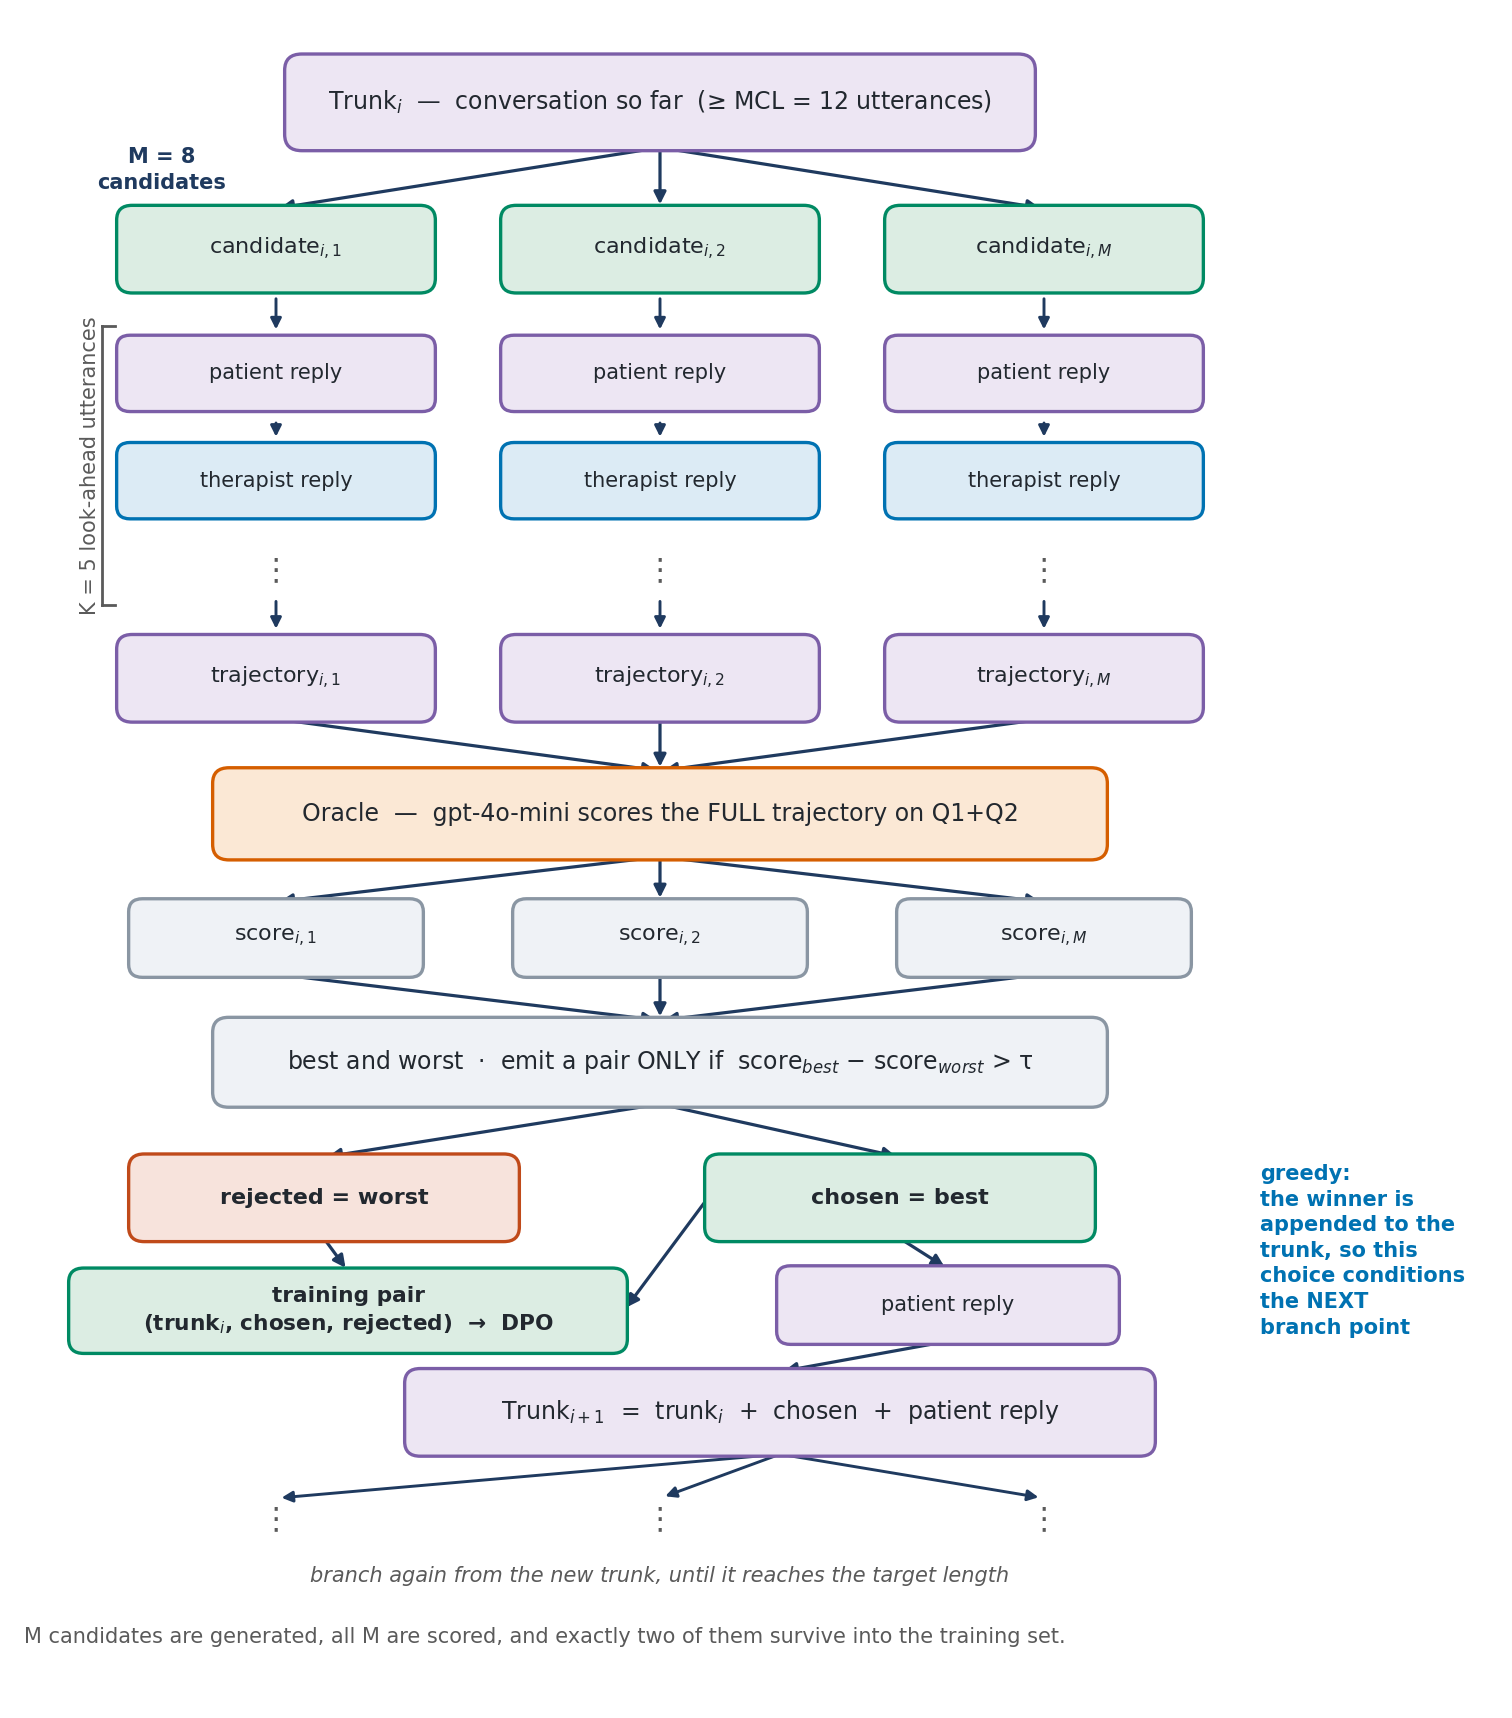
\includegraphics[width=\linewidth]{figures/method_pto_tree.png}
\end{subfigure}\hfill
\begin{subfigure}[t]{0.495\linewidth}
  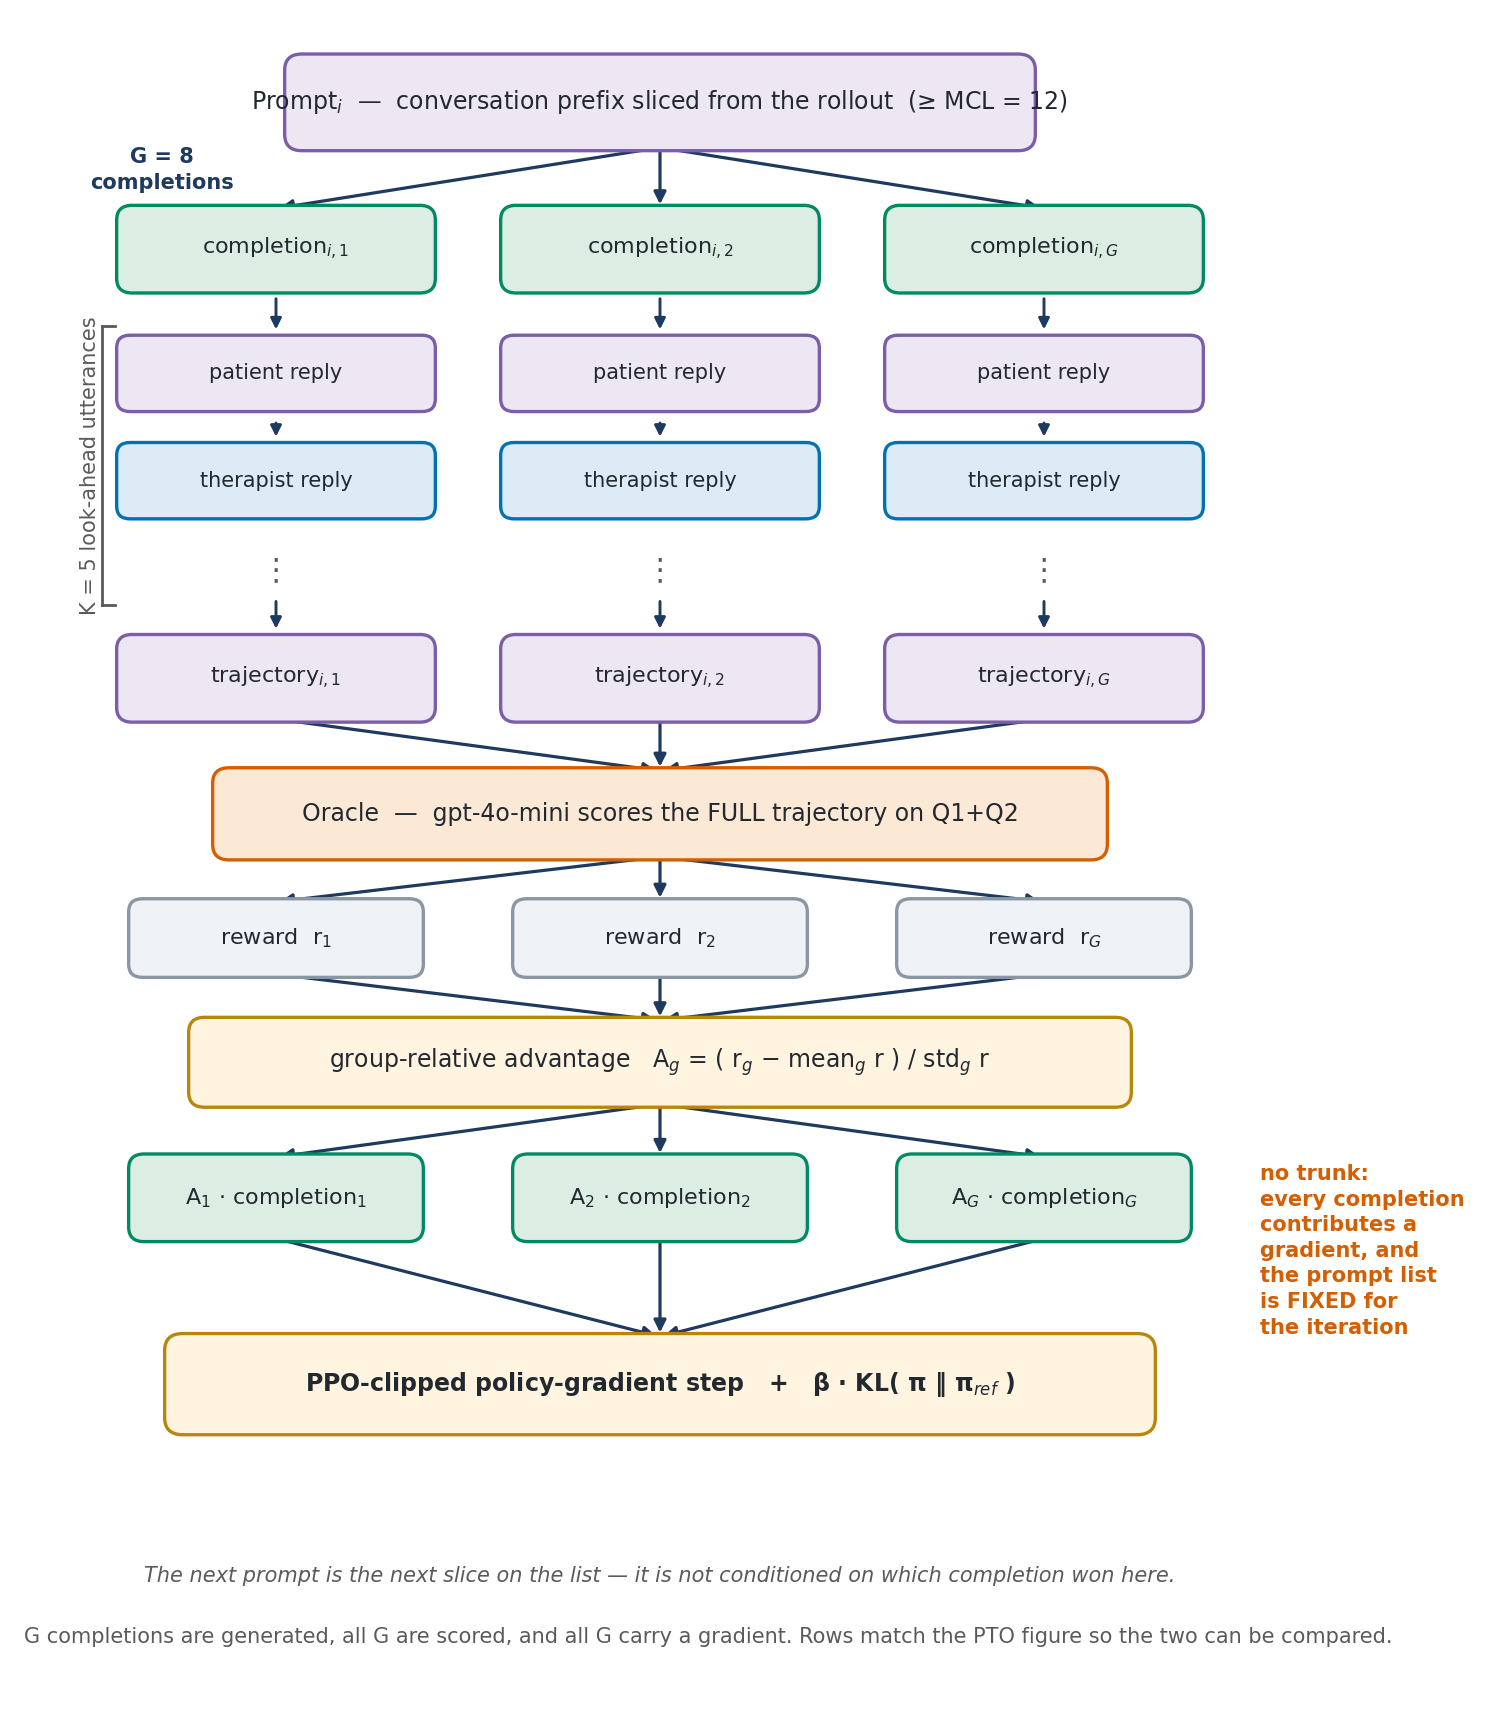
\includegraphics[width=\linewidth]{figures/method_grpo_group.png}
\end{subfigure}
\caption{The two optimizers over the same machinery. \textbf{Left:} \PTO\ grows a trunk by
appending the best of $M{=}8$ oracle-scored candidates and trains DPO on best-vs-worst pairs.
\textbf{Right:} \GRPO\ scores all $G{=}8$ siblings and trains on every one via a group-relative
advantage. In both, the $K$ lever changes only the transcript the oracle sees per candidate.}
\label{fig:schematics}
\end{figure}

\textbf{Evaluation and statistics.} Every model state $\times$ instrument is scored for all 96
conversations by two graders: the \textbf{training oracle} (\primaryjudge) and a \textbf{held-out
judge} (\heldoutjudge), a different model family that never played the patient and never touched
training. All contrasts are \textbf{persona-paired} (personas are reshuffled per iteration, so
pairing replays the shuffle rather than trusting file order), with Wilcoxon signed-rank tests,
Cohen's \dz, 2{,}000-resample percentile bootstrap intervals at a fixed seed, and Holm correction
within each family. The graders' \emph{levels} are never compared or averaged --- the held-out
judge is systematically harsher by 1.2--1.7 points, model-dependently --- only contrasts cross
graders. Compute is reported in \emph{reconstructed GPU-hours} from per-step artifact timestamps,
because in-process timing fields undercount resumed runs (Appendix~\ref{app:repro}).
